\documentclass[10pt,a4paper]{article}
\usepackage[utf8]{inputenc}
\usepackage{amsmath}
\usepackage{amsfonts}
\usepackage{amssymb}
\usepackage{amsthm}
\usepackage{float}
\usepackage{mathtools}
\usepackage{geometry}[margin=1in]
\usepackage{xspace}
\usepackage{tikz}
\usepackage{mathrsfs}
\usetikzlibrary{shapes, arrows, decorations.pathmorphing, ducks, automata}
\usepackage[parfill]{parskip}
\usepackage{subcaption}
\usepackage{stmaryrd}
\usepackage{marvosym}
\usepackage{dsfont}
\usepackage{pgfplots}
\usepackage{enumitem}
\usepackage{calc}
\usepackage{tikz-cd}
\usepackage{hyperref}

\hypersetup{
    colorlinks,
    citecolor=black,
    filecolor=black,
    linkcolor=black,
    urlcolor=black
}

\newcommand{\st}{\text{ s.t. }}
\newcommand{\contr}{\lightning}
\newcommand{\im}{\mathfrak{i}}
\newcommand{\R}{\mathbb{R}}
\newcommand{\Q}{\mathbb{Q}}
\newcommand{\C}{\mathbb{C}}
\newcommand{\F}{\mathbb{F}}
\newcommand{\K}{\mathbb{K}}
\newcommand{\N}{\mathbb{N}}
\newcommand{\Z}{\mathbb{Z}}
\renewcommand{\P}{\mathbb{P}}
\renewcommand{\H}{\mathds{H}}
\renewcommand{\O}{\mathcal{O}}
\newcommand{\A}{\mathbb{A}}
\newcommand{\D}{\mathbb{D}}
\newcommand{\nequiv}{\not\equiv}
\newcommand{\powset}{\mathcal{P}}
\renewcommand{\th}[1][th]{\textsuperscript{#1}\xspace}
\newcommand{\from}{\leftarrow}
\newcommand{\legendre}[2]{\left(\frac{#1}{#2}\right)}
\newcommand{\ow}{\text{otherwise}}
\newcommand{\imp}[2]{\underline{\textit{#1.}$\implies$\textit{#2.}}}
\let\oldexists\exists
\let\oldforall\forall
\renewcommand{\exists}{\oldexists\;}
\renewcommand{\forall}{\;\oldforall}
\renewcommand{\hat}{\widehat}
\renewcommand{\tilde}{\widetilde}
\newcommand{\one}{\mathds{1}}
\newcommand{\under}{\backslash}
\newcommand{\injection}{\hookrightarrow}
\newcommand{\surjection}{\twoheadrightarrow}
\newcommand{\jacobi}{\legendre}
\newcommand{\floor}[1]{\lfloor #1 \rfloor}
\newcommand{\ceil}[1]{\lceil #1 \rceil}
\newcommand{\cbrt}[1]{\sqrt[3]{#1}}
\renewcommand{\angle}[1]{\langle #1 \rangle}
\newcommand{\dbangle}[1]{\angle{\angle{#1}}}
\newcommand{\wrt}{\text{ w.r.t. }}

\newcommand*\circled[1]{\tikz[baseline=(char.base)]{
      \node[shape=circle,draw,inner sep=2pt] (char) {#1};}
}

\DeclareMathOperator{\ex}{ex}
\DeclareMathOperator{\id}{id}
\DeclareMathOperator{\upper}{Upper}
\DeclareMathOperator{\dom}{dom}
\DeclareMathOperator{\disc}{disc}
\DeclareMathOperator{\charr}{char}
\DeclareMathOperator{\Image}{im}
\DeclareMathOperator{\ord}{ord}
\DeclareMathOperator{\lcm}{lcm}
\DeclareMathOperator{\aut}{Aut}
\DeclareMathOperator{\diag}{diag}
\DeclareMathOperator{\stab}{stab}
\DeclareMathOperator{\trace}{trace}
\DeclareMathOperator{\ecl}{ecl}
\DeclareMathOperator{\Span}{Span}
\DeclareMathOperator{\Gal}{Gal}
\DeclareMathOperator{\Aut}{Aut}
\DeclareMathOperator{\Frob}{Frob}
\let\div\relax
\DeclareMathOperator{\div}{div}
\DeclareMathOperator{\Div}{Div}
\let\Re\relax
\let\Im\relax
\DeclareMathOperator{\Re}{\mathfrak{Re}}
\DeclareMathOperator{\Im}{\mathfrak{Im}}
\DeclareMathOperator{\Frac}{Frac}
\DeclareMathOperator{\Pic}{Pic}

\let\emph\relax
\DeclareTextFontCommand{\emph}{\bfseries\em}

\newtheorem{theorem}{Theorem}[section]
\newtheorem{lemma}[theorem]{Lemma}
\newtheorem{corollary}[theorem]{Corollary}
\newtheorem{proposition}[theorem]{Proposition}
\newtheorem{conjecture}[theorem]{Conjecture}
\newtheorem{definition}[theorem]{Definition}

\definecolor{burgundy}{rgb}{0.5, 0.0, 0.13}

\tikzset{sketch/.style={decorate,
 decoration={random steps, amplitude=1pt, segment length=5pt},
 line join=round, draw=black!80, very thick, fill=#1
}}

\pgfplotsset
  {
    compat                   = newest,
    every tick/.append style = thin,
    width= 0.95 \textwidth,
  }

\title{Complex Dynamics}
\begin{document}
\section{Introduction}
\subsection{Classical Motivation: Newton's Method}
Newton's method (also called Newton-Raphson) is an algorithm for finding roots of a polynomial. If $p(z)$ is a polynomial, then we construct the auxiliary function $f(z) = z - \frac{p(z)}{p'(z)}$. We then pick some value $z_0$ and we iterate, so that $z_{i+1} = f(z_i)$. Sometimes, depending on $p$ and $z_0$, this sequence converges to some $z$, so that $z = z-\frac{p(z)}{p'(z)}$, i.e. $p(z) = 0$. We can view this graphically for real values of $z$ as follows:

\begin{figure}[H]
  \centering
    \begin{tikzpicture}
      \begin{axis}[xmin = -3, xmax = 7, ymin = -2, ymax = 4, restrict y to domain=-10:10, axis lines=middle, xtick={-3,-2,...,7}, ytick={-1,0,...,4}, axis equal]
        \node[burgundy, circle, draw, fill, scale=0.1, label={[burgundy]below:$z_0$}] (a) at (4, 2.6875) {};
        \node[scale=0] (b) at (2.6875, 2.6875) {};
        \node[burgundy, circle, draw, fill, scale=0.1, label={[burgundy]below:$z_1$}] (c) at (2.6875, 1.8378) {};
        \node[scale=0] (d) at (1.8378, 1.8378) {};
        \node[scale=0] (e) at (1.8378, 1.3239) {};
        \node[scale=0] (f) at (1.3239, 1.3239) {};
        \node[scale=0] (g) at (1.3239, 1.0727) {};
        \node[scale=0] (h) at (1.0727, 1.0727) {};
        \node[scale=0] (i) at (1.0727, 1.0048) {};
        \node[scale=0] (j) at (1.0048, 1.0048) {};

        \draw[burgundy, ->] (a) edge (b) (b) edge (c) (c) edge (d) (d) edge (e) (e) edge (f);
        \draw[burgundy] (f) -- (g) -- (h) -- (i) -- (j);

        \addplot+[samples=100, mark=none, domain=-3:-0.24, blue] {(2*x^3+1)/(3*x^2)};
        \addplot+[samples=100, mark=none, domain=0.25:5, blue] {(2*x^3+1)/(3*x^2)} node[right, pos=1] {$f(x) = \frac{2x^3+1}{3x^2}$};
        \addplot+[red, mark=none] {x};
      \end{axis}
    \end{tikzpicture}
  \caption{Newton's method for $p(z) = z^3-1$}
\end{figure}

It's not too hard to see that, no matter our starting choice of $z_0$, this process will always eventually converge towards $z=1$, and that $p(1) = 0$.

If instead we consider this iteration for \emph{complex} values of $z_0$, we might converge to different roots of $p(z)$, since $p$ also has two complex roots. It turns out that the question of deciding which root we will converge to is not easy, and in fact we can see which root will be converged to in the following convergence diagram\footnote{Courtesy of \url{usefuljs.net/fractals/docs/newtonian_fractals.html}}
\begin{figure}[H]
  \centering
  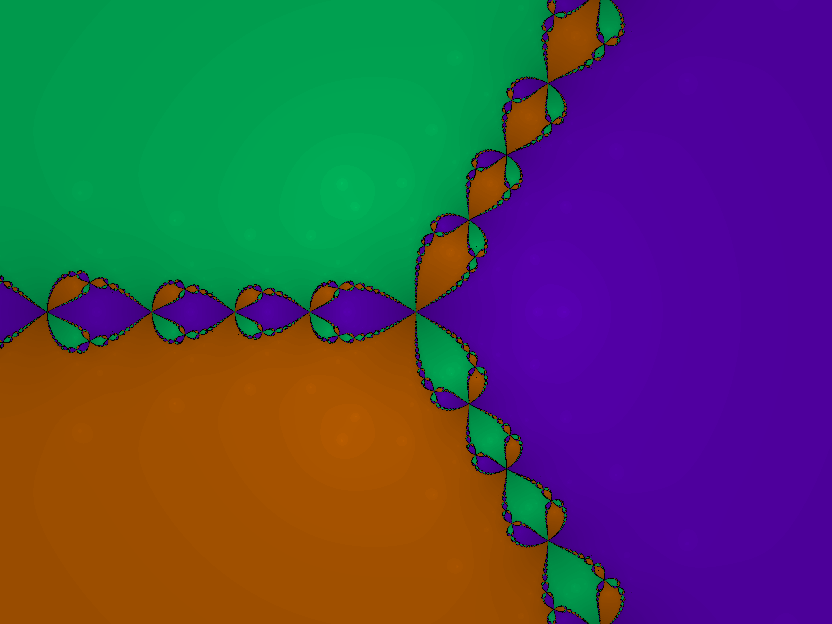
\includegraphics[width=0.95\textwidth]{compdyn01.png}
  \caption{Convergence diagram for $z^3-1$}
\end{figure}

We have many different stable behaviours of this dynamical system, but the boundary is very chaotic. For example, if we consider $p(z) = z^4-2z^2+9$, note that if $z \in \R$, then $f(z) \in \R$. However, the four roots of $p$ are all complex, and so Newton's method will fail to work for $z_0 \in \R$, and this can be seen in the following image:
\begin{figure}[H]
  \centering
  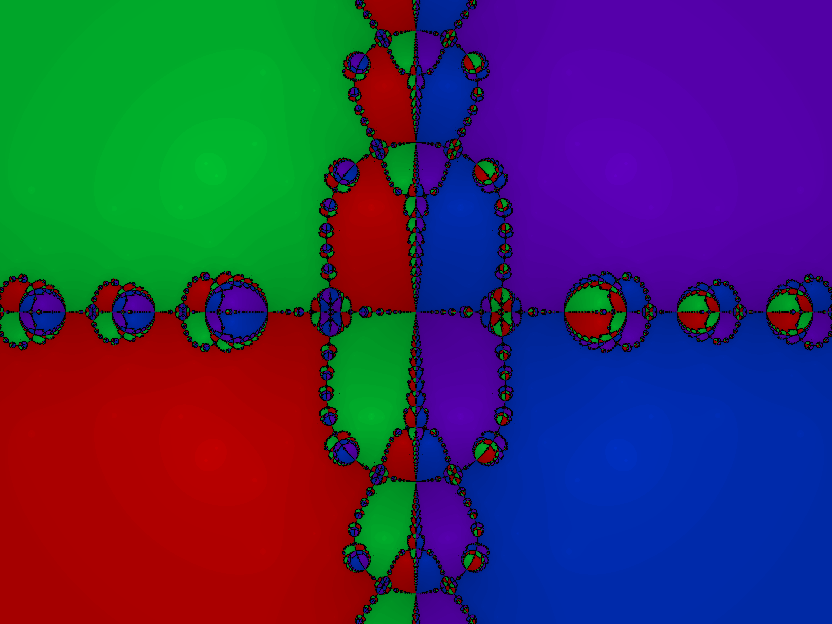
\includegraphics[width=0.95\textwidth]{compdyn02.png}
  \caption{Convergence diagram for $z^4-2z^2+9$}
\end{figure}

\subsection{Applications Motivation: Fixed Point Problems}
Gravitational Lensing: Suppose we have $n$ point masses in a plane perpendicular to the line of sight, and we are observing an object at the origin of this plane, identified with the complex plane. Call the points $z_1, \ldots, z_n$, with masses $\sigma_1, \ldots, \sigma_n$ respectively. Then the images of the object at the origin are the solutions to the \emph{lens equation} $z = \sum_{j=1}^n \frac{\sigma_j}{\bar{z} - \bar{z_j}}$. We see this for instance in the following image, courtesy of \texttt{Nasa}
\begin{figure}[H]
  \centering
  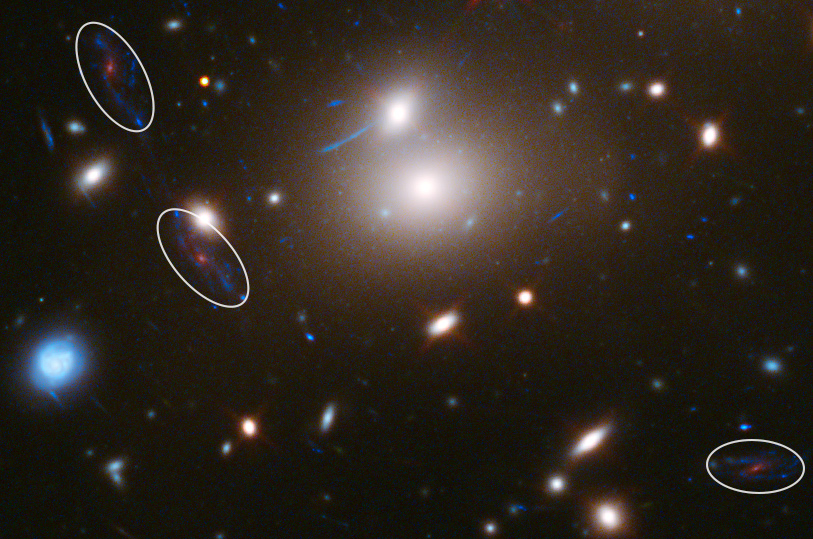
\includegraphics[width=0.95\textwidth]{compdyn03.jpg}
  \caption{The same galaxy appearing 3 times in an image captured by Hubble.}
\end{figure}

For example, if we have a point mass at the origin $n=1, z_1 = 0$. The lens equation gives us images of it at $z = \frac{\sigma_1}{\bar{z}}$, i.e. $|z|^2 = \sigma_1$. The solution is a circle, known as an \emph{Einstein ring}.
\begin{figure}[H]
  \centering
  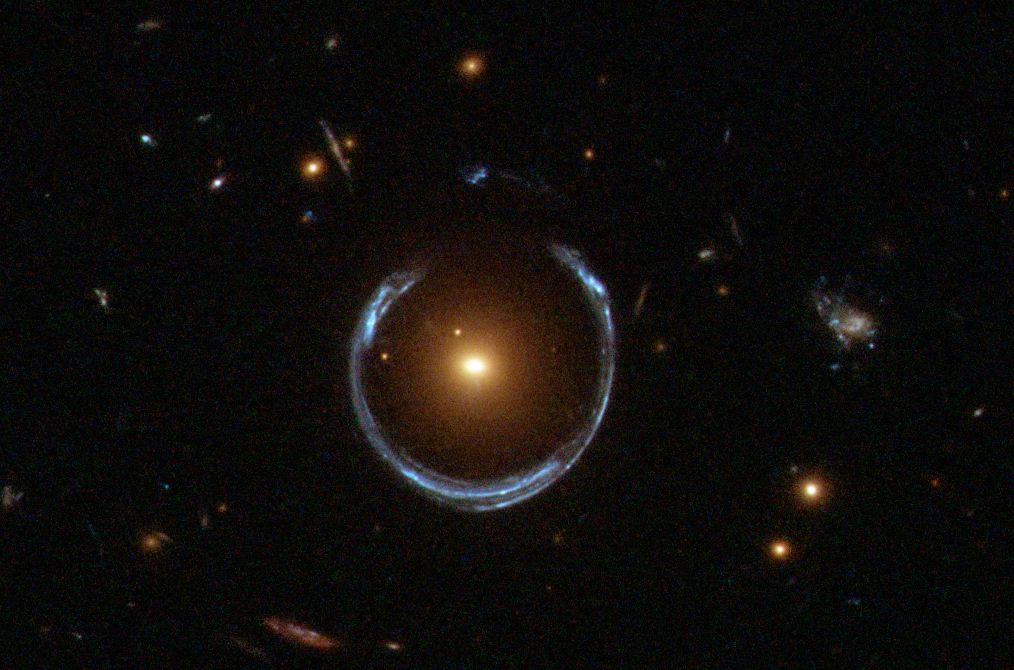
\includegraphics[width=0.95\textwidth]{compdyn04.jpg}
  \caption{An Einstein ring, captured by Hubble.}
\end{figure}

In general, we might want to ask how many images we will see for a give configuration, or perhaps a given number, of point masses.

Define $r(z) \coloneqq \sum_{j=1}^n \frac{\sigma_j}{z-z_j}$, and we are looking for solutions to $z = \overline{r(z)}$, i.e. fixed points of the (non-meromorphic) function $z \mapsto \overline{r(z)}$. These will be among the solutions of the (meromorphic) function $z\mapsto \overline{r(\overline{r(z)})} = r(r(z))$, of degree $n^2$. One can show that it suffices to bound the number of \emph{attracting} fixed points, which will be done in one of the main theorems of this course:

\begin{theorem}
Let $f(z)$ be a rational map of degree $d \geq 2$. Then $f$ has at most $2d-2$ attracting fixed points.
\end{theorem}

There are still open questions related to this application; for example, the following conjecture is still open despite its simplicity:
\begin{conjecture}[(Lee, Lerario, Lundberg)]
If $p$ is a polynomial of degree $n$, $q$ a polynomial of degree $m$, and $n>m$, then the number of solutions to $p(z) = \overline{q(z)}$ is bounded above by $2m(n-1)+n$.
\end{conjecture}

\subsection{Where We're Heading}
Define $f_c(z) \coloneqq z^2+c$, where $c \in \C$. \emph{The Mandelbrot Set} $M \coloneqq \{c \in \C : |f_c^n(0)|\nrightarrow\infty as n\to\infty\}$.
\begin{figure}[H]
  \centering
  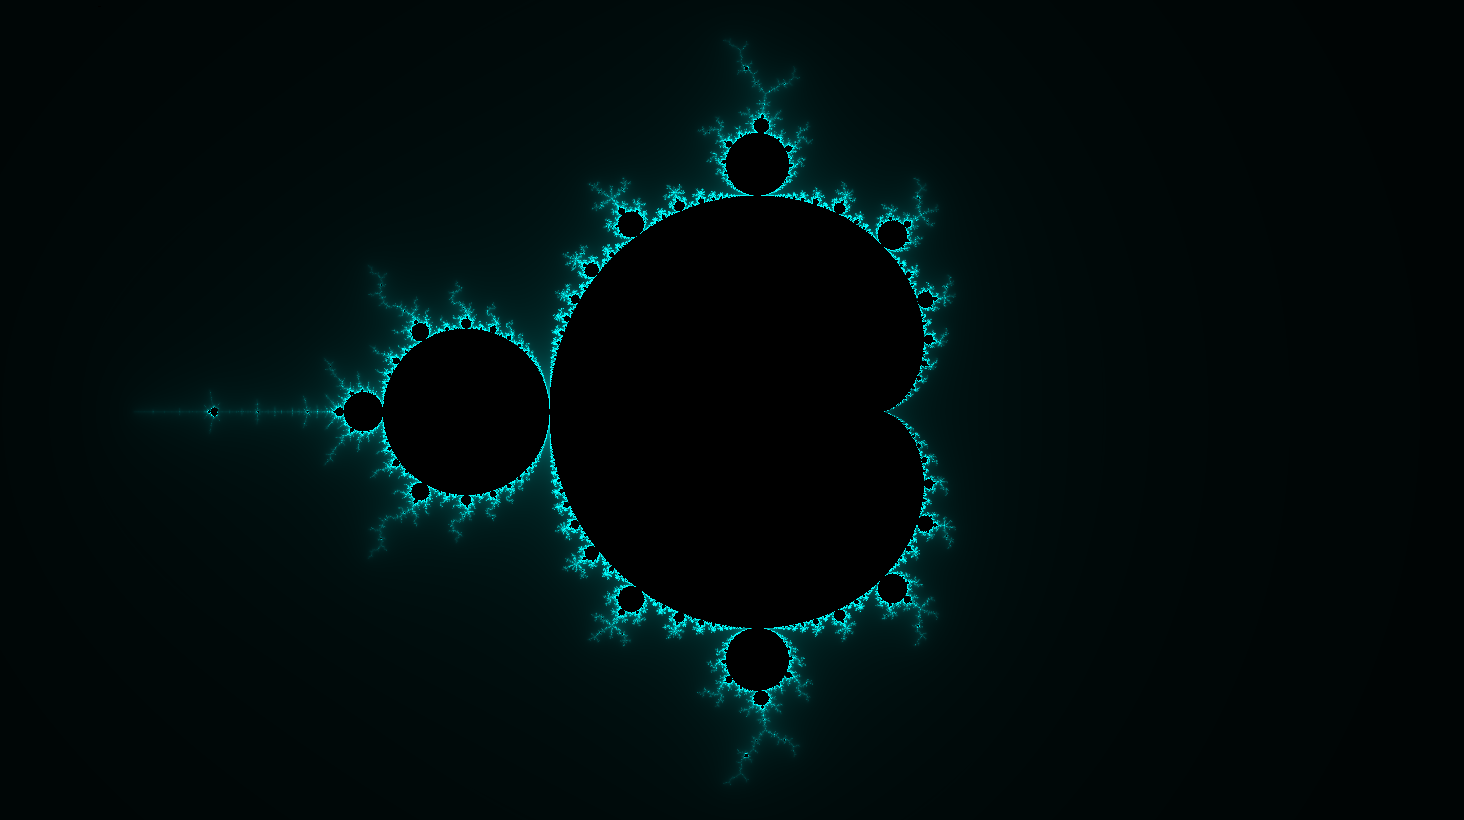
\includegraphics[width=0.95\textwidth]{compdyn05.png}
  \caption{The Mandelbrot set, generated by me.}
\end{figure}

\section{Complex Basics}
\subsection{The Riemann Sphere}
The \emph{Riemann Sphere} $\hat{\C}$ is the one-point compactification of $\C$, given by adding a point at $\infty$. The basis of this topology around $\infty$ are the complements of the closed discs in $\C$.

\begin{definition}
A \emph{domain} in the Riemann sphere is any open connected subset of $\hat{\C}$.
\end{definition}
We can then think about \emph{maps of the Riemann sphere}, which are rational maps of the form $f(z) = \frac{p(z)}{q(z)}$, where $p, q$ are polynomials with no common roots. We define the \emph{degree} of $f$ to be the maximum of $\deg p, \deg q$.

\begin{definition}
We say that $f : \hat{\C} \to \hat{\C}$ is \emph{holomorphic at $\infty$} if $f(1/z)$ is meromorphic on a neighbourhood of 0.
\end{definition}

\begin{lemma}[Identity Principle]
Let $f: D \to D$ be a holomorphic, non-constant map on a domain $D$ in $\hat{\C}$. Then for any $w \in D, f^{-1}(w)$ is discrete. In particular, if $D = \hat{\C}$, then $f^{-1}(w)$ is finite.
\end{lemma}
\begin{proof}
First, composing with a M\"obius map, we may assume $w = 0$. By the principle of isolated zeros, $\forall z \in \hat{\C}$, there is some disc $D_z \ni z$ such that either $f \equiv 0$ on  on $D_z$ or $f$ is nonzero on $D_z \setminus \{z\}$.

Let $V \coloneqq \bigcup_{f = 0 \text{ on } D_z} D_z$, $W \coloneqq \bigcup_{f \neq 0 \text{ on } D_z} D_z$

Then $V \cup W = D$, these sets are open, and $V \cap W = \emptyset$. Since $D$ is connected, $V$ and $W$ cannot disconnect $D$, so one of $V$ and $W$ is empty. $f$ is nonconstant, so $V = \emptyset$, and so the zeros are discrete. As $\hat{\C}$ is compact, any discrete subset is finite.
\end{proof}

\begin{proposition}
Let $f: \hat{\C} \to \hat{\C}$ be a holomorphic, non-constant map. Then $f$ is a non-constant rational function; that is, there exist $a_1, \ldots, a_m, b_1, \ldots b_n \in \C$, and $c \in \C^{\times}$ such that:
\begin{align*}
f(z) = \frac{c(z-a_1)\ldots(z-a_m)}{(z-b_1)\ldots(z-b_n)}
\end{align*}
\end{proposition}

\begin{proof}
Replace by $\frac{1}{f}$ if necessary to assume $f(\infty) \in \C$. By the identity principle, $f^{-1}(\infty)$ is a finite subset of $\C$. Call it $\{b_1, \ldots, b_n\}$. Near each $b_j$, we have a local expansion of $f$ as $f(z) = \sum_{i=-k}^\infty a_{j,i}(z-b_j)^i$. Set $Q_j(z) = \sum_{i=-k}^{-1} a_{j,i}(z-b_j)^i$, each $Q_j$ is a rational function and $g \coloneqq f - (Q_1 + \ldots + Q_n)$ has only removable singularities. So $g(\hat{\C}) \subseteq \C$. Since $\hat{\C}$ is compact, $g(\hat{\C})$ is a compact, proper, open subset of $\C$ $\contr$ (by Heine-Borel). Therefore $g$ is constant, and $f$ is rational.
\end{proof}

\subsection{The Derivative at Infinity}
Caution: there is not a globally well defined notion of a derivative of $f:\hat{\C} \to \hat{\C}$, since we can change coordinates in many different ways. However, if $f(\infty) = \infty$, then we do, as the local derivative is independent of choice of coordinates. In this case, we define $f'(\infty)$ to be the derivative at 0 of $\frac{1}{f(1/z)}$.
\end{document}
